\documentclass{standalone}
\usepackage{tikz}
\usetikzlibrary{patterns, positioning}

\begin{document}
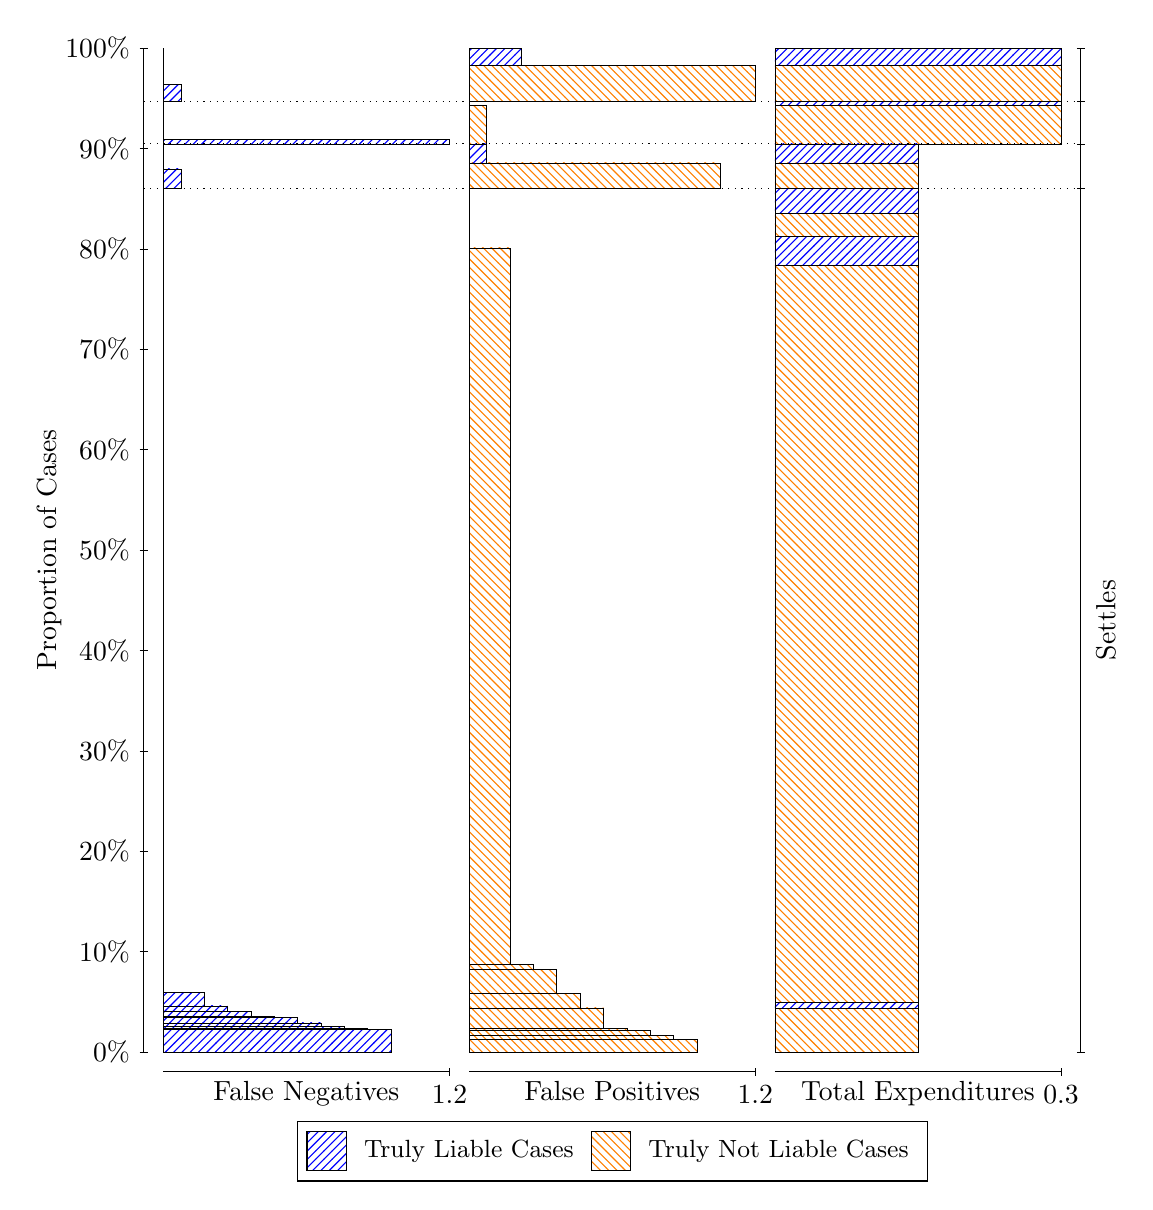
\begin{tikzpicture}
\draw[black, very thin] (1.5,1.75) -- (1.5,14.5);
\node[rotate=90, anchor=center] at (0.3, 8.125) {Proportion of Cases};
\draw[black, very thin] (1.45,1.75) -- (1.55,1.75);
\node[anchor=east] at (1.45, 1.75) {0\%};
\draw[black, very thin] (1.45,3.025) -- (1.55,3.025);
\node[anchor=east] at (1.45, 3.025) {10\%};
\draw[black, very thin] (1.45,4.3) -- (1.55,4.3);
\node[anchor=east] at (1.45, 4.3) {20\%};
\draw[black, very thin] (1.45,5.575) -- (1.55,5.575);
\node[anchor=east] at (1.45, 5.575) {30\%};
\draw[black, very thin] (1.45,6.85) -- (1.55,6.85);
\node[anchor=east] at (1.45, 6.85) {40\%};
\draw[black, very thin] (1.45,8.125) -- (1.55,8.125);
\node[anchor=east] at (1.45, 8.125) {50\%};
\draw[black, very thin] (1.45,9.4) -- (1.55,9.4);
\node[anchor=east] at (1.45, 9.4) {60\%};
\draw[black, very thin] (1.45,10.675) -- (1.55,10.675);
\node[anchor=east] at (1.45, 10.675) {70\%};
\draw[black, very thin] (1.45,11.95) -- (1.55,11.95);
\node[anchor=east] at (1.45, 11.95) {80\%};
\draw[black, very thin] (1.45,13.225) -- (1.55,13.225);
\node[anchor=east] at (1.45, 13.225) {90\%};
\draw[black, very thin] (1.45,14.5) -- (1.55,14.5);
\node[anchor=east] at (1.45, 14.5) {100\%};

\draw[black, very thin] (13.4,1.75) -- (13.4,14.5);
\draw[black, very thin] (13.35,1.75) -- (13.45,1.75);
\node[anchor=west] at (13.35, 1.75) {};
\draw[black, very thin] (13.35,12.72) -- (13.45,12.72);
\node[anchor=west] at (13.35, 12.72) {};
\draw[black, very thin] (13.35,13.284) -- (13.45,13.284);
\node[anchor=west] at (13.35, 13.284) {};
\draw[black, very thin] (13.35,13.82) -- (13.45,13.82);
\node[anchor=west] at (13.35, 13.82) {};
\draw[black, very thin] (13.35,14.5) -- (13.45,14.5);
\node[anchor=west] at (13.35, 14.5) {};

\draw[black, very thin, pattern color=blue, pattern=north east lines] (1.75,1.75) rectangle (4.6418,2.0396);
\draw[black, very thin, pattern color=blue, pattern=north east lines] (1.75,2.0396) rectangle (4.3452,2.0498);
\draw[black, very thin, pattern color=blue, pattern=north east lines] (1.75,2.0498) rectangle (4.0486,2.0757);
\draw[black, very thin, pattern color=blue, pattern=north east lines] (1.75,2.0757) rectangle (3.752,2.1182);
\draw[black, very thin, pattern color=blue, pattern=north east lines] (1.75,2.1182) rectangle (3.4554,2.1893);
\draw[black, very thin, pattern color=blue, pattern=north east lines] (1.75,2.1893) rectangle (3.1588,2.2046);
\draw[black, very thin, pattern color=blue, pattern=north east lines] (1.75,2.2046) rectangle (2.8622,2.2696);
\draw[black, very thin, pattern color=blue, pattern=north east lines] (1.75,2.2696) rectangle (2.5656,2.3362);
\draw[black, very thin, pattern color=blue, pattern=north east lines] (1.75,2.3362) rectangle (2.269,2.5079);
\draw[black, very thin, pattern color=orange, pattern=north west lines] (1.75,2.5079) rectangle (1.75,12.72);
\draw[black, very thin, pattern color=blue, pattern=north east lines] (1.75,12.72) rectangle (1.9724,12.965);
\draw[black, very thin, pattern color=orange, pattern=north west lines] (1.75,12.965) rectangle (1.75,13.284);
\draw[black, very thin, pattern color=blue, pattern=north east lines] (1.75,13.284) rectangle (5.3833,13.335);
\draw[black, very thin, pattern color=orange, pattern=north west lines] (1.75,13.335) rectangle (1.75,13.82);
\draw[black, very thin, pattern color=blue, pattern=north east lines] (1.75,13.82) rectangle (1.9724,14.042);
\draw[black, very thin, pattern color=orange, pattern=north west lines] (1.75,14.042) rectangle (1.75,14.5);
\draw[black, very thin, pattern color=orange, pattern=north west lines] (5.6333,1.75) rectangle (8.5252,1.9084);
\draw[black, very thin, pattern color=orange, pattern=north west lines] (5.6333,1.9084) rectangle (8.2286,1.9621);
\draw[black, very thin, pattern color=orange, pattern=north west lines] (5.6333,1.9621) rectangle (7.932,2.0268);
\draw[black, very thin, pattern color=orange, pattern=north west lines] (5.6333,2.0268) rectangle (7.6354,2.0469);
\draw[black, very thin, pattern color=orange, pattern=north west lines] (5.6333,2.0469) rectangle (7.3388,2.3104);
\draw[black, very thin, pattern color=orange, pattern=north west lines] (5.6333,2.3104) rectangle (7.0422,2.4925);
\draw[black, very thin, pattern color=orange, pattern=north west lines] (5.6333,2.4925) rectangle (6.7456,2.802);
\draw[black, very thin, pattern color=orange, pattern=north west lines] (5.6333,2.802) rectangle (6.449,2.8609);
\draw[black, very thin, pattern color=orange, pattern=north west lines] (5.6333,2.8609) rectangle (6.1524,11.962);
\draw[black, very thin, pattern color=blue, pattern=north east lines] (5.6333,11.962) rectangle (5.6333,12.72);
\draw[black, very thin, pattern color=orange, pattern=north west lines] (5.6333,12.72) rectangle (8.8218,13.04);
\draw[black, very thin, pattern color=blue, pattern=north east lines] (5.6333,13.04) rectangle (5.8558,13.284);
\draw[black, very thin, pattern color=orange, pattern=north west lines] (5.6333,13.284) rectangle (5.8558,13.769);
\draw[black, very thin, pattern color=blue, pattern=north east lines] (5.6333,13.769) rectangle (5.6333,13.82);
\draw[black, very thin, pattern color=orange, pattern=north west lines] (5.6333,13.82) rectangle (9.2667,14.278);
\draw[black, very thin, pattern color=blue, pattern=north east lines] (5.6333,14.278) rectangle (6.3007,14.5);
\draw[black, very thin, pattern color=orange, pattern=north west lines] (9.5167,1.75) rectangle (11.333,2.3005);
\draw[black, very thin, pattern color=blue, pattern=north east lines] (9.5167,2.3005) rectangle (11.333,2.379);
\draw[black, very thin, pattern color=orange, pattern=north west lines] (9.5167,2.379) rectangle (11.333,11.744);
\draw[black, very thin, pattern color=blue, pattern=north east lines] (9.5167,11.744) rectangle (11.333,12.105);
\draw[black, very thin, pattern color=orange, pattern=north west lines] (9.5167,12.105) rectangle (11.333,12.402);
\draw[black, very thin, pattern color=blue, pattern=north east lines] (9.5167,12.402) rectangle (11.333,12.72);
\draw[black, very thin, pattern color=orange, pattern=north west lines] (9.5167,12.72) rectangle (11.333,13.04);
\draw[black, very thin, pattern color=blue, pattern=north east lines] (9.5167,13.04) rectangle (11.333,13.284);
\draw[black, very thin, pattern color=orange, pattern=north west lines] (9.5167,13.284) rectangle (13.15,13.769);
\draw[black, very thin, pattern color=blue, pattern=north east lines] (9.5167,13.769) rectangle (13.15,13.82);
\draw[black, very thin, pattern color=orange, pattern=north west lines] (9.5167,13.82) rectangle (13.15,14.278);
\draw[black, very thin, pattern color=blue, pattern=north east lines] (9.5167,14.278) rectangle (13.15,14.5);
\draw[black, dotted] (1.5,12.72) -- (13.4,12.72);
\draw[black, dotted] (1.5,13.284) -- (13.4,13.284);
\draw[black, dotted] (1.5,13.82) -- (13.4,13.82);
\draw[black, very thin] (1.75,1.5) -- (5.3833,1.5);
\node[anchor=north] at (3.5667, 1.5) {False Negatives};
\draw[black, very thin] (5.3833,1.45) -- (5.3833,1.55);
\node[anchor=north] at (5.3833, 1.45) {1.2};

\draw[black, very thin] (5.6333,1.5) -- (9.2667,1.5);
\node[anchor=north] at (7.45, 1.5) {False Positives};
\draw[black, very thin] (9.2667,1.45) -- (9.2667,1.55);
\node[anchor=north] at (9.2667, 1.45) {1.2};

\draw[black, very thin] (9.5167,1.5) -- (13.15,1.5);
\node[anchor=north] at (11.333, 1.5) {Total Expenditures};
\draw[black, very thin] (13.15,1.45) -- (13.15,1.55);
\node[anchor=north] at (13.15, 1.45) {0.3};

\node[black, centered, rotate=90] at (13.72, 7.2351) {Settles};




\draw (7.449999999999999,1.5) node[draw=none] (baseCoordinate) {};
\begin{scope}[align=center]
        \matrix[scale=0.5, draw=black, below=0.5cm of baseCoordinate, nodes={draw}, column sep=0.1cm]{
            \node[rectangle, draw, minimum width=0.5cm, minimum height=0.5cm, pattern=north east lines, pattern color=blue] {}; &
            \node[draw=none, font=\small] (B) {Truly Liable Cases}; &
            \node[rectangle, draw, minimum width=0.5cm, minimum height=0.5cm, pattern=north west lines, pattern color=orange] {}; &
            \node[draw=none, font=\small] (B) {Truly Not Liable Cases}; \\
            };
\end{scope}

\end{tikzpicture}
\end{document}